\documentclass[11pt]{article}
\usepackage{amsmath, amssymb, mathtools, bm}
\usepackage{physics}
\usepackage{tikz}
\usetikzlibrary{arrows.meta, calc, positioning, decorations.pathmorphing, patterns, 3d}
\usepackage{pgfplots}
\pgfplotsset{compat=1.18}
\usepackage[margin=2.3cm]{geometry}
\usepackage{siunitx}
\usepackage{booktabs}
\usepackage{hyperref}
\usepackage{braket}

\newcommand{\de}{\mathrm{d}}
\newcommand{\pd}[2]{\frac{\partial #1}{\partial #2}}
\newcommand{\pdd}[2]{\frac{\partial^{2} #1}{\partial #2^{2}}}
\newcommand{\Lap}{\nabla^{2}}
\newcommand{\kB}{k_{\mathrm{B}}}
\newcommand{\NA}{N_{\mathrm{A}}}
\newcommand{\TF}{T_{\mathrm{F}}}
\newcommand{\TD}{T_{\mathrm{D}}}
\newcommand{\EF}{E_{\mathrm{F}}}
\newcommand{\eF}{\epsilon_{\mathrm{F}}}
\newcommand{\muB}{\mu_{\mathrm{B}}}

\title{B6: Condensed-Matter Physics --- 2024 Model Solutions}
\author{Trinity Term 2024 (Paper A13485W1)}
\date{}

\begin{document}
\maketitle

%==========================================================
\section*{Question 1 --- Sodium under pressure: bcc--fcc transition and X-ray diffraction}

\textbf{Problem.} Na is bcc at $p=0$ ($a_0=\SI{4.27}{\angstrom}$) and undergoes a first-order bcc$\to$fcc transition at $p_c=\SI{65}{GPa}$, with $a=\SI{2.90}{\angstrom}$ just below and $a'=\SI{3.65}{\angstrom}$ just above. Powder XRD uses $\lambda=\SI{0.43}{\angstrom}$; molar mass $M=\SI{23}{g\,mol^{-1}}$.

\subsection*{(a)(i)--(ii) Conventional unit cells and atoms per cell}

\begin{center}
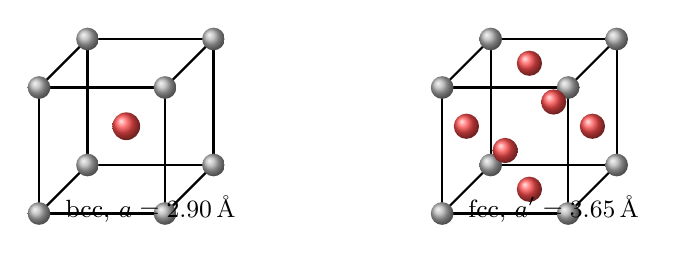
\begin{tikzpicture}[scale=1.6]
\begin{scope}[xshift=0cm]
\draw[thick] (0,0,0)--(1,0,0)--(1,1,0)--(0,1,0)--cycle;
\draw[thick] (0,0,1)--(1,0,1)--(1,1,1)--(0,1,1)--cycle;
\draw[thick] (0,0,0)--(0,0,1); \draw[thick] (1,0,0)--(1,0,1);
\draw[thick] (1,1,0)--(1,1,1); \draw[thick] (0,1,0)--(0,1,1);
\foreach \x/\y/\z in {0/0/0,1/0/0,1/1/0,0/1/0,0/0/1,1/0/1,1/1/1,0/1/1}{
  \shade[ball color=gray!60] (\x,\y,\z) circle (0.09);
}
\shade[ball color=red!70] (0.5,0.5,0.5) circle (0.11);
\node at (0.5,-0.35,0) {\small bcc, $a=\SI{2.90}{\angstrom}$};
\end{scope}
\begin{scope}[xshift=3.2cm]
\draw[thick] (0,0,0)--(1,0,0)--(1,1,0)--(0,1,0)--cycle;
\draw[thick] (0,0,1)--(1,0,1)--(1,1,1)--(0,1,1)--cycle;
\draw[thick] (0,0,0)--(0,0,1); \draw[thick] (1,0,0)--(1,0,1);
\draw[thick] (1,1,0)--(1,1,1); \draw[thick] (0,1,0)--(0,1,1);
\foreach \x/\y/\z in {0/0/0,1/0/0,1/1/0,0/1/0,0/0/1,1/0/1,1/1/1,0/1/1}{
  \shade[ball color=gray!60] (\x,\y,\z) circle (0.09);
}
\foreach \x/\y/\z in {0.5/0.5/0,0.5/0.5/1,0.5/0/0.5,0.5/1/0.5,0/0.5/0.5,1/0.5/0.5}{
  \shade[ball color=red!70] (\x,\y,\z) circle (0.10);
}
\node at (0.5,-0.35,0) {\small fcc, $a'=\SI{3.65}{\angstrom}$};
\end{scope}
\end{tikzpicture}
\end{center}

Count corners (each shared $\times 1/8$) plus interior atoms:
\[
n_{\mathrm{bcc}} = 8\times\tfrac{1}{8} + 1 = 2.
\]
\[
n_{\mathrm{fcc}} = 8\times\tfrac{1}{8} + 6\times\tfrac{1}{2} = 4.
\]
\[
\boxed{\ n_{\mathrm{bcc}}=2,\quad n_{\mathrm{fcc}}=4.\ }
\]

\subsection*{(a)(iii)--(iv) The $(111)$ plane and nearest-neighbour distance in it}

bcc $(111)$ contains only the three corners (the body-centre atom is off the plane); side $=\sqrt 2 a$:
\[
d^{\,(111)}_{\mathrm{bcc}} = \sqrt{2}\times\SI{2.90}{\angstrom} = \SI{4.10}{\angstrom}.
\]
fcc $(111)$ is close-packed with separation $a'/\sqrt 2$:
\[
d^{\,(111)}_{\mathrm{fcc}} = \SI{3.65}{\angstrom}/\sqrt{2} = \SI{2.58}{\angstrom}.
\]

\begin{center}
\begin{tikzpicture}[scale=0.9]
\begin{scope}
\draw[gray] (0,0)--(4.10,0)--(2.05,3.55)--cycle;
\foreach \p in {(0,0),(4.10,0),(2.05,3.55)} \shade[ball color=gray!70] \p circle (0.13);
\node at (2.05,-0.6) {\small bcc $(111)$: $d=\sqrt{2}a=\SI{4.10}{\angstrom}$};
\end{scope}
\begin{scope}[xshift=7cm]
\foreach \i in {0,1,2,3}{
  \foreach \j in {0,1,2,3}{
    \pgfmathsetmacro{\xx}{2.58*(\i + 0.5*\j)}
    \pgfmathsetmacro{\yy}{2.58*0.866*\j}
    \shade[ball color=red!70] (\xx,\yy) circle (0.13);
  }
}
\node at (3.0,-0.6) {\small fcc $(111)$: $d=a'/\sqrt{2}=\SI{2.58}{\angstrom}$};
\end{scope}
\end{tikzpicture}
\end{center}

\[
\boxed{\ d_{\mathrm{bcc}}^{(111)}=\SI{4.10}{\angstrom},\quad d_{\mathrm{fcc}}^{(111)}=\SI{2.58}{\angstrom}.\ }
\]

\subsection*{(b)(i) Diffraction selection rules and reflection positions}

Bragg + cubic spacing $d_{hk\ell}=a/\sqrt{h^2+k^2+\ell^2}$:
\begin{equation}
\sin\theta = \frac{\lambda}{2a}\sqrt{N},\qquad N\equiv h^2+k^2+\ell^2.
\label{eq:braggcubic}
\end{equation}
Selection rules:
\begin{equation}
\boxed{\ \text{bcc: }h+k+\ell\text{ even};\quad \text{fcc: }h,k,\ell\text{ all even or all odd.}\ }
\label{eq:selrules}
\end{equation}
Allowed $N$ sequences:
\[
N_{\mathrm{bcc}}: 2,4,6,8,\dots\ (hk\ell)=110,200,211,220,\dots
\]
\[
N_{\mathrm{fcc}}: 3,4,8,11,12,\dots\ (hk\ell)=111,200,220,311,222,\dots
\]
Window $2\theta<\SI{25}{\degree}$ requires $\sin\theta<0.2164$.

bcc, $\lambda/(2a)=0.07414$, $\sqrt N<2.919$, $N\le 8$:
\begin{equation}
\begin{aligned}
(110): N=2,&\quad 2\theta=\SI{12.04}{\degree};\\
(200): N=4,&\quad 2\theta=\SI{17.04}{\degree};\\
(211): N=6,&\quad 2\theta=\SI{20.90}{\degree};\\
(220): N=8,&\quad 2\theta=\SI{24.18}{\degree}.
\end{aligned}
\label{eq:bccpeaks}
\end{equation}
fcc, $\lambda/(2a')=0.05890$, $\sqrt N<3.674$, $N\le 12$:
\begin{equation}
\begin{aligned}
(111): N=3,&\quad 2\theta=\SI{11.71}{\degree};\\
(200): N=4,&\quad 2\theta=\SI{13.53}{\degree};\\
(220): N=8,&\quad 2\theta=\SI{19.18}{\degree};\\
(311): N=11,&\quad 2\theta=\SI{22.55}{\degree};\\
(222): N=12,&\quad 2\theta=\SI{23.55}{\degree}.
\end{aligned}
\label{eq:fccpeaks}
\end{equation}

\subsection*{(b)(ii) Sketch of the two diffraction patterns}

\begin{center}
\begin{tikzpicture}[xscale=0.42, yscale=1.5]
\draw[->] (0,0)--(28,0) node[right] {$2\theta$ ($^\circ$)};
\draw[->] (0,0)--(0,1.6) node[above] {$I$};
\foreach \x in {0,5,10,15,20,25} \draw (\x,-0.05)--(\x,0.05) node[below=2pt]{\scriptsize \x};
\foreach \x/\hkl in {12.04/110,17.04/200,20.90/211,24.18/220}{
  \draw[blue, very thick] (\x,0)--(\x,1.0);
  \node[blue, above, rotate=90, anchor=west] at (\x,1.0) {\scriptsize (\hkl)};
}
\node[blue] at (3,0.9) {\textbf{bcc}};
\end{tikzpicture}
\end{center}

\begin{center}
\begin{tikzpicture}[xscale=0.42, yscale=1.5]
\draw[->] (0,0)--(28,0) node[right] {$2\theta$ ($^\circ$)};
\draw[->] (0,0)--(0,1.6) node[above] {$I$};
\foreach \x in {0,5,10,15,20,25} \draw (\x,-0.05)--(\x,0.05) node[below=2pt]{\scriptsize \x};
\foreach \x/\hkl in {11.71/111,13.53/200,19.18/220,22.55/311,23.55/222}{
  \draw[red, very thick] (\x,0)--(\x,1.0);
  \node[red, above, rotate=90, anchor=west] at (\x,1.0) {\scriptsize (\hkl)};
}
\node[red] at (3,0.9) {\textbf{fcc}};
\end{tikzpicture}
\end{center}

\subsection*{(b)(iii) Lattice parameter at $p_1=\SI{100}{GPa}$}

Third allowed fcc reflection $(220)$ at $2\theta=\SI{19.18}{\degree}$ shifts up by $\SI{1.20}{\degree}$:
\[
2\theta^{(1)}_{220} = 19.18+1.20 = \SI{20.38}{\degree}.
\]
Take half:
\[
\sin\theta^{(1)}_{220} = \sin(\SI{10.19}{\degree}) = 0.17681.
\]
Apply \eqref{eq:braggcubic} with $\sqrt N=2\sqrt 2$:
\[
a'_1 = \frac{\lambda\sqrt N}{2\sin\theta^{(1)}_{220}} = \frac{0.43\times 2\sqrt 2}{2\times 0.17681}\,\si{\angstrom}.
\]
\begin{equation}
\boxed{\ a'_1 = \SI{3.44}{\angstrom}.\ }
\label{eq:a1box}
\end{equation}

\subsection*{(c) Hard-sphere atomic radius and density change at $p_c$}

bcc touch along body diagonal $\sqrt 3 a = 4r$:
\[
r_{\mathrm{bcc}} = \tfrac{\sqrt 3}{4}\times \SI{2.90}{\angstrom} = \SI{1.256}{\angstrom}.
\]
fcc touch along face diagonal $\sqrt 2 a' = 4r$:
\[
r_{\mathrm{fcc}} = \tfrac{\sqrt 2}{4}\times \SI{3.65}{\angstrom} = \SI{1.291}{\angstrom}.
\]
Number density $n=n_{\mathrm{cell}}/a^3$:
\[
n_b = 2/(2.90)^3\,\si{\angstrom^{-3}} = 8.20\times 10^{28}\,\si{m^{-3}}.
\]
\[
n_f = 4/(3.65)^3\,\si{\angstrom^{-3}} = 8.23\times 10^{28}\,\si{m^{-3}}.
\]
Mass density $\rho=nM/\NA$:
\[
\rho_{\mathrm{bcc}} = \frac{8.20\times 10^{28}\times 23\times 10^{-3}}{6.022\times 10^{23}}\,\si{kg\,m^{-3}} = \SI{3133}{kg\,m^{-3}}.
\]
\[
\rho_{\mathrm{fcc}} = \frac{8.226\times 10^{28}\times 23\times 10^{-3}}{6.022\times 10^{23}}\,\si{kg\,m^{-3}} = \SI{3142}{kg\,m^{-3}}.
\]
Fractional change:
\begin{equation}
\boxed{\ \Delta\rho/\rho_{\mathrm{bcc}} = +0.31\%,\quad \Delta\rho \approx +\SI{9}{kg\,m^{-3}}.\ }
\label{eq:drhobox}
\end{equation}

\subsection*{(d) Compressibility of the bcc phase between ambient and $p_c$}

Per-atom volume $v=a^3/2$. Treat $\beta=-(1/V)\partial V/\partial p$ constant; integrate:
\[
V(p) = V_0 e^{-\beta p}.
\]
Solve for $\beta$ at $p=p_c$:
\[
\beta = -\frac{1}{p_c}\ln\frac{V}{V_0} = -\frac{3}{p_c}\ln\frac{a}{a_0}.
\]
Evaluate $\ln(2.90/4.27)=-0.3866$, $p_c=\SI{65e9}{Pa}$:
\[
\beta_{\mathrm{bcc}} = \frac{3\times 0.3866}{6.5\times 10^{10}}\,\si{Pa^{-1}}.
\]
\begin{equation}
\boxed{\ \beta_{\mathrm{bcc}} = \SI{1.78e-11}{Pa^{-1}}.\ }
\label{eq:betabox}
\end{equation}

\subsection*{(e) Mass of sodium that fits in the pressure cell}

Cylindrical volume:
\[
V_{\mathrm{cyl}} = \pi(50\times 10^{-6})^2\times 10^{-3}\,\si{m^3} = \SI{7.854e-12}{m^3}.
\]
$35\%$ void $\Rightarrow$ Na occupies $0.65\,V_{\mathrm{cyl}}$:
\[
V_{\mathrm{Na}} = 0.65\times \SI{7.854e-12}{m^3} = \SI{5.10e-12}{m^3}.
\]
Ambient bcc density with $a_0^3=\SI{77.85e-30}{m^3}$:
\[
\rho_0 = \frac{2\times 23\times 10^{-3}}{6.022\times 10^{23}\times 77.85\times 10^{-30}}\,\si{kg\,m^{-3}} = \SI{981}{kg\,m^{-3}}.
\]
Mass:
\[
m_{\mathrm{Na}} = 981\times 5.10\times 10^{-12}\,\si{kg}.
\]
\begin{equation}
\boxed{\ m_{\mathrm{Na}} \approx \SI{5.0e-9}{kg} \approx \SI{5}{ng}.\ }
\label{eq:massbox}
\end{equation}

%==========================================================
\section*{Question 2 --- Heat capacity of YbMg$_2$Bi$_2$ in 3D and 2D}

\textbf{Problem.} 3D molar heat capacity is $C=z\NA\kB[(\pi^2/2)(T/\TF)+(12\pi^4/5)(T/\TD)^3]$ at low $T$, saturating at high $T$. (a) Identify $z$ from the saturation. (b) Justify each term, extract $\TF,\TD$ from $C/T$ vs $T^2$, find cross-over $T^\ast$. (c) For a 2D film with two in-plane polarisations, find $g_{\mathrm{ph}}^{(2)}(\omega)$, the high-$T$ limit, and the low-$T$ form $C=AT+BT^\delta$ with $A(g(\EF))$, $B(\omega_D)$. Use $\int_0^\infty x^3/(e^x-1)\,\de x=\pi^4/15$, $\int_0^\infty x^2/(e^x-1)\,\de x=2\zeta(3)\simeq 2.4$.

\subsection*{(a) Origin of the high-$T$ saturation and Dulong--Petit limit}

Equipartition for $3N$ classical modes:
\[
C_{\mathrm{lat}}^{(\infty)} = 3N\kB.
\]
Per mole of formula units, $N=z\NA$:
\[
C^{(\infty)} = 3zR.
\]
Read $C^{(\infty)}\simeq \SI{120}{J\,mol^{-1}\,K^{-1}}$ from figure:
\[
z = 120/(3\times 8.314) \approx 4.8.
\]
\begin{equation}
\boxed{\ z=5\text{ atoms per formula unit.}\ }
\label{eq:zbox}
\end{equation}

\subsection*{(b)(i) Justification of the two terms}

\textbf{Linear electronic term.} Sommerfeld expansion to leading order in $T/\TF$:
\begin{equation}
U_{\mathrm{el}}(T) = U_{\mathrm{el}}(0) + \tfrac{\pi^2}{6}g(\EF)(\kB T)^2.
\label{eq:Uel}
\end{equation}
Differentiate:
\begin{equation}
C_{\mathrm{el}} = \tfrac{\pi^2}{3}g(\EF)\kB^2 T \equiv \gamma T.
\label{eq:CelGamma}
\end{equation}
Free-electron-like: $g(\EF) = 3N_e/(2\kB\TF)$. Substitute:
\[
C_{\mathrm{el}} = \tfrac{\pi^2}{3}\cdot\tfrac{3N_e}{2\kB\TF}\kB^2 T = \tfrac{\pi^2}{2}N_e\kB\,\tfrac{T}{\TF}.
\]
Identify $N_e=z\NA$ to recover the stated prefactor.

\textbf{Cubic Debye term.} 3D phonon DOS (3 acoustic branches):
\begin{equation}
g_{\mathrm{ph}}(\omega) = \frac{3V\omega^2}{2\pi^2 v_s^3}.
\label{eq:gph3D}
\end{equation}
Internal energy:
\[
U_{\mathrm{ph}}(T) = \int_0^{\omega_D}\frac{\hbar\omega}{e^{\hbar\omega/\kB T}-1}g_{\mathrm{ph}}(\omega)\,\de\omega.
\]
Substitute $x=\hbar\omega/\kB T$:
\[
U_{\mathrm{ph}}(T) = \frac{3V}{2\pi^2 v_s^3 \hbar^3}(\kB T)^4 \int_0^{x_D}\frac{x^3}{e^x-1}\,\de x.
\]
Low $T$, extend the upper limit to $\infty$:
\[
U_{\mathrm{ph}}(T) \approx \frac{3V}{2\pi^2 v_s^3 \hbar^3}(\kB T)^4 \cdot \frac{\pi^4}{15}.
\]
Eliminate $V/v_s^3$ via $\omega_D^3 = 6\pi^2 N v_s^3/V$:
\[
\frac{V}{v_s^3} = \frac{6\pi^2 N\hbar^3}{(\kB\TD)^3}.
\]
Substitute:
\[
U_{\mathrm{ph}}(T) = \tfrac{3\pi^4}{5}N\kB\,\frac{T^4}{\TD^3}.
\]
Differentiate, use $N=z\NA$:
\begin{equation}
\boxed{\ C_{\mathrm{ph}}(T) = \tfrac{12\pi^4}{5}z\NA\kB\,\frac{T^3}{\TD^3}.\ }
\label{eq:CphlowT}
\end{equation}

\subsection*{(b)(ii) Reading $\TF$ and $\TD$ from the $C/T$ vs $T^2$ plot}

Model:
\begin{equation}
\frac{C}{T} = \gamma + \beta T^2,\quad \gamma=\frac{\pi^2 z R}{2\TF},\ \beta=\frac{12\pi^4 zR}{5\TD^3}.
\label{eq:CTline}
\end{equation}
Read intercept $\gamma\simeq\SI{0.30}{J\,mol^{-1}\,K^{-2}}$, slope $\beta\simeq \SI{1.6e-3}{J\,mol^{-1}\,K^{-4}}$.

Solve for $\TF$:
\[
\TF = \frac{\pi^2\times 5\times 8.314}{2\times 0.30}\,\si{K} \approx \SI{684}{K}.
\]
\begin{equation}
\boxed{\ \TF \approx \SI{7e2}{K}.\ }
\label{eq:TFbox}
\end{equation}

Solve for $\TD$:
\[
\TD^3 = \frac{12\pi^4\times 5\times 8.314}{5\times 1.6\times 10^{-3}}\,\si{K^3} = 6.07\times 10^5\,\si{K^3}.
\]
Cube root:
\[
\TD \approx \SI{195}{K}.
\]
\begin{equation}
\boxed{\ \TD \approx \SI{2e2}{K}.\ }
\label{eq:TDbox}
\end{equation}

\subsection*{(b)(iii) Cross-over temperature $T^\ast$}

Equate the two contributions:
\[
\tfrac{\pi^2}{2}\,\frac{T^*}{\TF} = \tfrac{12\pi^4}{5}\!\left(\frac{T^*}{\TD}\right)^3.
\]
Solve for $(T^*)^2$:
\[
(T^*)^2 = \frac{5\TD^3}{24\pi^2 \TF}.
\]
Plug numbers:
\[
(T^*)^2 = \frac{5\times 195^3}{24\pi^2\times 684}\,\si{K^2} = 229\,\si{K^2}.
\]
\begin{equation}
\boxed{\ T^* \approx \SI{15}{K}.\ }
\label{eq:Tstarbox}
\end{equation}

\subsection*{(c)(i) 2D phonon density of states}

Two in-plane polarisations, mode density $A/(2\pi)^2$ per polarisation, $\omega=v_s|\mathbf q|$:
\[
g_{\mathrm{ph}}^{(2)}(\omega)\,\de\omega = 2\cdot\frac{A}{(2\pi)^2}\cdot 2\pi q\,\de q.
\]
Insert $q=\omega/v_s$:
\[
g_{\mathrm{ph}}^{(2)}(\omega)\,\de\omega = \frac{A\omega}{\pi v_s^2}\,\de\omega.
\]
\begin{equation}
\boxed{\ g_{\mathrm{ph}}^{(2)}(\omega) = \frac{A\omega}{\pi v_s^2}.\ }
\label{eq:g2Dbox}
\end{equation}

\subsection*{(c)(ii) High-$T$ Dulong--Petit in 2D}

Total in-plane modes $=2N$, each $\kB$:
\[
C^{(\infty)}_{2D} = 2N\kB.
\]
Per mole, $N=z\NA$:
\begin{equation}
\boxed{\ C^{(\infty)}_{\mathrm{molar}} = 2zR = 10R \approx \SI{83}{J\,mol^{-1}\,K^{-1}}.\ }
\label{eq:DP2Dbox}
\end{equation}

\subsection*{(c)(iii) Low-$T$ form $C=AT+BT^\delta$ in 2D}

Phonon energy with $g_{\mathrm{ph}}^{(2)}$:
\[
U_{\mathrm{ph}}^{(2)}(T) = \int_0^{\omega_D}\frac{\hbar\omega}{e^{\hbar\omega/\kB T}-1}\,\frac{A\omega}{\pi v_s^2}\,\de\omega.
\]
Substitute $x=\hbar\omega/\kB T$:
\[
U_{\mathrm{ph}}^{(2)}(T) = \frac{A}{\pi v_s^2 \hbar^2}(\kB T)^3\int_0^{x_D}\frac{x^2}{e^x-1}\,\de x.
\]
Low $T$, extend the upper limit to $\infty$:
\[
U_{\mathrm{ph}}^{(2)}(T) \approx \frac{A}{\pi v_s^2 \hbar^2}(\kB T)^3 \cdot 2\zeta(3).
\]
Differentiate:
\begin{equation}
\boxed{\ C^{(2)}_{\mathrm{ph}}(T) = \frac{6\zeta(3)A\kB^3}{\pi v_s^2 \hbar^2}\,T^2 \equiv B T^\delta,\quad \delta=2.\ }
\label{eq:CphLowT2D}
\end{equation}

\subsection*{(c)(iv) Identification of $A$ in terms of $g(\EF)$, and $B$ in terms of $\omega_D$}

Sommerfeld result \eqref{eq:CelGamma} is dimension-independent:
\begin{equation}
\boxed{\ A = \tfrac{\pi^2}{3}\kB^2\,g(\EF).\ }
\label{eq:Aresult}
\end{equation}

Debye condition (total in-plane modes $=2N$):
\[
2N = \int_0^{\omega_D}\frac{A\omega}{\pi v_s^2}\,\de\omega = \frac{A\omega_D^2}{2\pi v_s^2}.
\]
Rearrange:
\[
\frac{A}{\pi v_s^2} = \frac{4N}{\omega_D^2}.
\]
Substitute into \eqref{eq:CphLowT2D}:
\[
C^{(2)}_{\mathrm{ph}} = \frac{6\zeta(3)\kB^3}{\hbar^2}\cdot\frac{4N\,T^2}{\omega_D^2} = \frac{24\zeta(3)N\kB^3}{\hbar^2\omega_D^2}\,T^2.
\]
Per mole, $N=z\NA$:
\begin{equation}
\boxed{\ B = \frac{24\zeta(3)\,z\NA\kB^3}{\hbar^2\omega_D^2}.\ }
\label{eq:Bbox}
\end{equation}

%==========================================================
\section*{Question 3 --- Tight-binding band on a 2D square lattice}

\textbf{Problem.} 2D square lattice (parameter $a$), tight-binding $\epsilon(k_x,k_y)=\epsilon_0+2t\cos k_xa+2t\cos k_ya$, $t>0$. Find dispersion along $\Gamma\to X\to M$, bandwidth, contours, effective masses; the linear $\eF=\eF'+\alpha N/A$ near the band minimum and $g(\epsilon)=\beta A$; for $A_{\mathrm{FS}}/A_{\mathrm{BZ}}=1/100$ at $a=\SI{3.5}{\angstrom}$, find $n_{2D}$ and Hall voltage.

\subsection*{(a)(i) Band dispersion along $\Gamma\to X\to M$}

Endpoint values:
\[
\epsilon(\Gamma)=\epsilon_0+4t,\quad \epsilon(X)=\epsilon_0,\quad \epsilon(M)=\epsilon_0-4t.
\]

\begin{center}
\begin{tikzpicture}[xscale=2.0, yscale=0.7]
\draw[->] (0,-5.5)--(0,5.5) node[above]{$\epsilon-\epsilon_0$};
\draw[->] (-0.1,0)--(3.3,0) node[right]{};
\draw[blue, very thick, domain=0:1.5, samples=80, smooth] plot (\x,{2*(1+cos(\x/1.5*pi r))});
\draw[blue, very thick, domain=1.5:3.0, samples=80, smooth] plot (\x,{2*(-1+cos((\x-1.5)/1.5*pi r))});
\draw[dashed, gray] (1.5,-5)--(1.5,5);
\draw[dashed, gray] (3.0,-5)--(3.0,5);
\node[circle,fill,inner sep=1.2pt,label=above right:{$+4t$}] at (0,4) {};
\node[circle,fill,inner sep=1.2pt,label=above right:{$0$}] at (1.5,0) {};
\node[circle,fill,inner sep=1.2pt,label=below right:{$-4t$}] at (3,-4) {};
\node[below] at (0,-0.2) {$\Gamma$};
\node[below] at (1.5,-0.2) {$X$};
\node[below] at (3,-0.2) {$M$};
\end{tikzpicture}
\end{center}

\subsection*{(a)(ii) Bandwidth}

\begin{equation}
\boxed{\ W = \epsilon_{\max}-\epsilon_{\min} = 8t.\ }
\label{eq:Wbox}
\end{equation}

\subsection*{(a)(iii) Constant-energy contours}

Expand around $M=(\pi/a,\pi/a)$, $\mathbf k=\mathbf K_M+\mathbf q$, $\cos(\pi+qa)\simeq -1+(qa)^2/2$:
\begin{equation}
\epsilon(\mathbf k) \simeq \epsilon_0-4t + ta^2(q_x^2+q_y^2).
\label{eq:expM}
\end{equation}
Expand around $\Gamma$, $\cos(qa)\simeq 1-(qa)^2/2$:
\begin{equation}
\epsilon(\mathbf k) \simeq \epsilon_0+4t - ta^2(q_x^2+q_y^2).
\label{eq:expGamma}
\end{equation}
Both circular. Half-filling $\epsilon=\epsilon_0$: $\cos k_xa=-\cos k_ya \Rightarrow k_xa = \pm(\pi - k_ya)$, a square rotated $45^\circ$.

\begin{center}
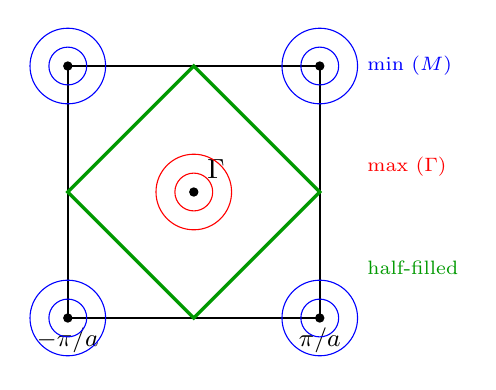
\begin{tikzpicture}[scale=1.6]
\draw[thick] (-1,-1) rectangle (1,1);
\node[below] at (1,-1) {\small $\pi/a$};
\node[below] at (-1,-1) {\small $-\pi/a$};
\node[circle,fill,inner sep=1.2pt,label=above right:{$\Gamma$}] at (0,0) {};
\node[circle,fill,inner sep=1.2pt] at (1,1) {};
\node[circle,fill,inner sep=1.2pt] at (-1,1) {};
\node[circle,fill,inner sep=1.2pt] at (1,-1) {};
\node[circle,fill,inner sep=1.2pt] at (-1,-1) {};
\foreach \r in {0.15,0.30}{
  \draw[blue] (1,1) circle (\r); \draw[blue] (-1,1) circle (\r);
  \draw[blue] (1,-1) circle (\r); \draw[blue] (-1,-1) circle (\r);
}
\foreach \r in {0.15,0.30}{
  \draw[red] (0,0) circle (\r);
}
\draw[green!60!black, very thick] (1,0)--(0,1)--(-1,0)--(0,-1)--cycle;
\node[red, right] at (1.3,0.2) {\scriptsize max ($\Gamma$)};
\node[blue, right] at (1.3,1.0) {\scriptsize min ($M$)};
\node[green!60!black, right] at (1.3,-0.6) {\scriptsize half-filled};
\end{tikzpicture}
\end{center}

\subsection*{(a)(iv) Effective masses near band edges}

From \eqref{eq:expM}, $\partial^2\epsilon/\partial q^2=2ta^2$:
\[
m^*_{\mathrm{min}} = \frac{\hbar^2}{2ta^2} > 0.
\]
From \eqref{eq:expGamma}, $\partial^2\epsilon/\partial q^2=-2ta^2$:
\[
m^*_{\mathrm{max}} = -\frac{\hbar^2}{2ta^2} < 0.
\]
\begin{equation}
\boxed{\ m^*_{\mathrm{min}} = +\frac{\hbar^2}{2ta^2},\qquad m^*_{\mathrm{max}} = -\frac{\hbar^2}{2ta^2}.\ }
\label{eq:meffbox}
\end{equation}

\subsection*{(b)(i)--(ii) $\eF(N/A)$ near the band minimum}

Parabolic band, $m^*=\hbar^2/(2ta^2)$. Count $\mathbf k$-states inside contour, factor 2 for spin:
\[
N(\eF) = 2\cdot\frac{A}{(2\pi)^2}\cdot \pi q_F^2.
\]
From \eqref{eq:expM}: $ta^2 q_F^2 = \eF-(\epsilon_0-4t)$. Substitute:
\[
\frac{N}{A} = \frac{q_F^2}{2\pi} = \frac{\eF-\epsilon_0+4t}{2\pi t a^2}.
\]
Solve for $\eF$:
\begin{equation}
\boxed{\ \eF = (\epsilon_0-4t) + 2\pi t a^2\,\frac{N}{A},\quad \eF'=\epsilon_0-4t,\ \alpha = 2\pi t a^2.\ }
\label{eq:eFlinear}
\end{equation}

\subsection*{(b)(iii) Density of states near the band minimum}

Differentiate $N$ with respect to $\eF$:
\[
g(\epsilon) = \pd{N}{\epsilon} = \frac{A}{2\pi t a^2}.
\]
\begin{equation}
\boxed{\ \beta = \frac{1}{2\pi t a^2}.\ }
\label{eq:gbox}
\end{equation}

\subsection*{(c)(i) Carrier density for $A_{\mathrm{FS}}/A_{\mathrm{BZ}}=1/100$}

BZ area $A_{\mathrm{BZ}}=(2\pi/a)^2$. Spin factor 2 over $\mathbf k$-cell:
\[
\frac{N}{A} = 2\cdot\frac{A_{\mathrm{FS}}}{(2\pi)^2} = \frac{2}{100}\cdot\frac{(2\pi/a)^2}{(2\pi)^2}.
\]
Simplify:
\[
\frac{N}{A} = \frac{1}{50 a^2}.
\]
For $a=\SI{3.5e-10}{m}$:
\[
n_{2D} = \frac{1}{50\times(3.5\times 10^{-10})^2}\,\si{m^{-2}}.
\]
\begin{equation}
\boxed{\ n_{2D} = \SI{1.63e17}{m^{-2}}.\ }
\label{eq:nbox}
\end{equation}

\subsection*{(c)(ii) Hall voltage}

Hall coefficient (single carrier, magnitude):
\[
R_H^{(2D)} = \frac{1}{n_{2D}\,e}.
\]
Hall field per unit width:
\[
V_H = \frac{j_x B_z}{n_{2D}\,e}.
\]
Plug $j_x=\SI{1.0e-5}{A\,m^{-1}}$, $B_z=\SI{1}{T}$:
\[
V_H = \frac{1.0\times 10^{-5}\times 1}{1.63\times 10^{17}\times 1.602\times 10^{-19}}\,\si{V}.
\]
Evaluate denominator:
\[
1.63\times 10^{17}\times 1.602\times 10^{-19} = 2.61\times 10^{-2}.
\]
Final:
\begin{equation}
\boxed{\ V_H \approx \SI{3.8e-4}{V} \approx \SI{0.38}{mV}.\ }
\label{eq:VHbox}
\end{equation}

%==========================================================
\section*{Question 4 --- Magnetism: Hund's rules, mean-field BCC ferromagnet}

\textbf{Problem.} (a) Hund's rules for Mn$^{2+}$ ($3d^5$), Tb$^{3+}$ ($4f^8$); $T=0$ moments. (b) $S=1/2$ Heisenberg + Zeeman on bcc (edge $a$): mean-field $B_{\mathrm{mf}}$, self-consistent $M$, Curie--Weiss $\chi$, $\Theta=T_C$, find $J_1$ for $T_C=\SI{30}{K}$. (c) Same on simple cubic with $T_C'=\SI{20}{K}$; find $J_1'$; sketch $\chi^{-1}(T)$.

\subsection*{(a)(i) Hund's rules for Mn$^{2+}$ ($3d^5$) and Tb$^{3+}$ ($4f^8$)}

\textbf{Mn$^{2+}$, $3d^5$.} Five $d$ electrons, one in each $m_\ell\in\{-2,\dots,2\}$:
\[
S = 5\times\tfrac12 = \tfrac52,\qquad L = \sum m_\ell = 0.
\]
Half-filled, $J=L+S$ or $|L-S|$ both give:
\[
J = \tfrac52.
\]
Land\'e factor:
\[
g_J = \tfrac32 + \frac{(5/2)(7/2)-0}{2(5/2)(7/2)} = 2.
\]
\begin{equation}
\boxed{\ \mathrm{Mn^{2+}}:\ S=\tfrac52,\ L=0,\ J=\tfrac52,\ g_J=2.\ }
\label{eq:Mnbox}
\end{equation}

\textbf{Tb$^{3+}$, $4f^8$.} Seven aligned, eighth pairs into $m_\ell=+3$:
\[
S = \tfrac{7}{2}-\tfrac12 = 3,\qquad L = 0+3 = 3.
\]
More than half full, $J=L+S$:
\[
J = 6.
\]
Land\'e factor:
\[
g_J = \tfrac32 + \frac{12-12}{2\cdot 6\cdot 7} = \tfrac32.
\]
\begin{equation}
\boxed{\ \mathrm{Tb^{3+}}:\ S=3,\ L=3,\ J=6,\ g_J=\tfrac32.\ }
\label{eq:Tbbox}
\end{equation}

\subsection*{(a)(ii) Saturation magnetic moment at $T=0$}

$m=g_J J\,\muB$:
\[
m_{\mathrm{Mn^{2+}}} = 2\times\tfrac52\,\muB = 5\,\muB.
\]
\[
m_{\mathrm{Tb^{3+}}} = \tfrac32\times 6\,\muB = 9\,\muB.
\]
\begin{equation}
\boxed{\ m_{\mathrm{Mn^{2+}}} = 5\,\muB,\qquad m_{\mathrm{Tb^{3+}}} = 9\,\muB.\ }
\label{eq:msatbox}
\end{equation}

\subsection*{(b)(i) Mean-field effective field on a bcc site}

bcc coordination $z=8$. Replace $\mathbf S_j\to\langle\mathbf S\rangle$ in the Heisenberg sum:
\begin{equation}
\mathcal H_i^{\mathrm{MF}} = -J_1 z\langle\mathbf S\rangle\cdot\mathbf S_i + g\muB\mathbf B\cdot\mathbf S_i \equiv g\muB\mathbf B_{\mathrm{mf}}\cdot\mathbf S_i.
\label{eq:HMF}
\end{equation}
Read off:
\[
\mathbf B_{\mathrm{mf}} = \mathbf B - \frac{J_1 z}{g\muB}\langle\mathbf S\rangle.
\]
Use $\mathbf M=-ng\muB\langle\mathbf S\rangle$, $n=2/a^3$:
\[
\langle\mathbf S\rangle = -\frac{\mathbf M}{ng\muB}.
\]
Substitute:
\[
\mathbf B_{\mathrm{mf}} = \mathbf B + \frac{J_1 z}{(g\muB)^2 n}\mathbf M \equiv \mathbf B + \lambda\mathbf M.
\]
Insert $z=8$, $n=2/a^3$:
\begin{equation}
\boxed{\ \lambda = \frac{4 J_1 a^3}{(g\muB)^2}.\ }
\label{eq:lambdabox}
\end{equation}

\subsection*{(b)(ii) Self-consistent magnetisation}

Single $S=1/2$ in $B_{\mathrm{mf}}$:
\[
Z = 2\cosh\!\left(\frac{g\muB B_{\mathrm{mf}}}{2\kB T}\right).
\]
Average projection $\tfrac12\tanh(\cdot)$, multiply by moment density $ng\muB$:
\[
M = \tfrac{ng\muB}{2}\tanh\!\left(\frac{g\muB B_{\mathrm{mf}}}{2\kB T}\right) \equiv M_0\tanh\!\left(\frac{g\muB B_{\mathrm{mf}}}{2\kB T}\right).
\]
Insert $n=2/a^3$:
\begin{equation}
\boxed{\ M_0 = \frac{g\muB}{a^3}.\ }
\label{eq:M0box}
\end{equation}

\subsection*{(b)(iii) Curie--Weiss susceptibility above $T_C$}

Expand $\tanh x\approx x$ for small $M$:
\[
M \simeq M_0\cdot\frac{g\muB(B+\lambda M)}{2\kB T}.
\]
Collect $M$:
\[
M\!\left(1 - \frac{M_0 g\muB \lambda}{2\kB T}\right) = \frac{M_0 g\muB B}{2\kB T}.
\]
Identify $\chi=M/B$:
\[
\chi = \frac{M_0 g\muB/(2\kB)}{T - M_0 g\muB \lambda/(2\kB)} \equiv \frac{C}{T-\Theta}.
\]
Substitute $M_0,\lambda$ from \eqref{eq:M0box},\eqref{eq:lambdabox}:
\[
\Theta = \frac{g\muB}{a^3}\cdot g\muB\cdot\frac{4J_1 a^3}{(g\muB)^2}\cdot\frac{1}{2\kB} = \frac{2J_1}{\kB}.
\]
\[
C = \frac{(g\muB)^2}{2\kB a^3}.
\]
\begin{equation}
\boxed{\ \Theta = \frac{2J_1}{\kB},\qquad C = \frac{(g\muB)^2}{2\kB a^3}.\ }
\label{eq:CWbox}
\end{equation}

\subsection*{(b)(iv) Relation $\Theta = T_C$}

$B=0$ self-consistent equation $M=M_0\tanh(g\muB\lambda M/(2\kB T))$. Non-zero solution emerges when slope at $M=0$ equals one:
\[
\frac{M_0 g\muB \lambda}{2\kB T_C} = 1.
\]
Identical to the pole condition in $\chi$:
\begin{equation}
\boxed{\ T_C = \Theta = \frac{2J_1}{\kB}.\ }
\label{eq:TCbox}
\end{equation}

\subsection*{(b)(v) Numerical $J_1$ for $T_C=\SI{30}{K}$}

\[
J_1 = \frac{\kB T_C}{2} = \frac{1.381\times 10^{-23}\times 30}{2}\,\si{J}.
\]
\begin{equation}
\boxed{\ J_1 \approx \SI{2.07e-22}{J} \approx \SI{1.3}{meV},\quad J_1/\kB \approx \SI{15}{K}.\ }
\label{eq:J1box}
\end{equation}

\subsection*{(c)(i) $J_1'$ for the simple-cubic lattice with $T_C'=\SI{20}{K}$}

Simple cubic: $z'=6$, $n'=1/a^3$. Repeat (b)(i)--(iii):
\[
\lambda' = \frac{6J_1' a^3}{(g\muB)^2},\qquad M_0' = \frac{g\muB}{2a^3}.
\]
Compute $\Theta'$:
\[
\Theta' = \frac{M_0' g\muB \lambda'}{2\kB} = \frac{3J_1'}{2\kB}.
\]
Set $T_C'=\Theta'$ and solve:
\[
J_1' = \frac{2\kB T_C'}{3} = \frac{2\times 1.381\times 10^{-23}\times 20}{3}\,\si{J}.
\]
\begin{equation}
\boxed{\ J_1' \approx \SI{1.84e-22}{J} \approx \SI{1.15}{meV},\quad J_1'/\kB \approx \SI{13.3}{K}.\ }
\label{eq:J1pbox}
\end{equation}

\subsection*{(c)(ii) Sketch of $\chi^{-1}(T)$ for both materials}

$\chi^{-1}=(T-\Theta)/C$, slope $1/C$, $T$-intercept $\Theta$. With $C_{\mathrm{bcc}}=(g\muB)^2/(2\kB a^3)$ and $C_{\mathrm{sc}}=(g\muB)^2/(4\kB a^3)$, the sc slope is twice the bcc slope.

\begin{center}
\begin{tikzpicture}[xscale=0.10, yscale=0.85]
\draw[->] (0,0)--(110,0) node[right]{$T$ (K)};
\draw[->] (0,0)--(0,4.8) node[above]{$\chi^{-1}$ (a.u.)};
\foreach \x in {0,20,30,50,75,100} \draw (\x,-0.07)--(\x,0.07) node[below=2pt]{\scriptsize \x};
\draw[blue, very thick, domain=30:105] plot (\x,{0.04*(\x-30)});
\draw[red, very thick, domain=20:105] plot (\x,{0.08*(\x-20)});
\node[circle,fill,blue,inner sep=1.2pt] at (30,0) {};
\node[circle,fill,red,inner sep=1.2pt] at (20,0) {};
\node[circle,fill,blue,inner sep=1.2pt] at (105,3.0) {};
\node[circle,fill,red,inner sep=1.2pt] at (105,6.8) {};
\node[blue, right] at (105, 3.0) {\small bcc, $T_C=30$\,K};
\node[red, right] at (105, 4.2) {\small sc, $T_C'=20$\,K};
\draw[dashed] (30,0)--(30,-0.3); \draw[dashed] (20,0)--(20,-0.3);
\end{tikzpicture}
\end{center}

\end{document}
